


\begin{frame}{Introducing Myself}
   \begin{block}{Education}
    \begin{itemize}
     \item Master's Degrees in Microelectronics and Mathematics
     \item Doctoral Degree in Microelectronics
     \item Home University: TU Wien
    \end{itemize}

   \vspace*{-2cm}
   \begin{flushright}
     
\includegraphics[width=0.15\textwidth]{figures/TU-Signet}
   \end{flushright}

   \end{block}



   \begin{block}{Interests}
    \begin{itemize}
     \item Efficient Numerics on Modern Hardware
     \item High-level APIs
     \item Semiconductor Device Simulation
    \end{itemize}

   \end{block}

   \begin{block}{Contact}
    \begin{itemize}
     \item Email: rupp@mcs.anl.gov
     \item Web: http://www.karlrupp.net/
     \item Find me at: Google+, Twitter, LinkedIn
    \end{itemize}
   \end{block}

\end{frame}





%% Table of Contents

%% 100x myth



%%%%%%% GPUs: Disillusion %%%%%%%

\begin{frame}{Hardware Specifications}
 \begin{block}{Peak FLOP/s} \end{block}
 \begin{center} \vspace*{-0.9cm} 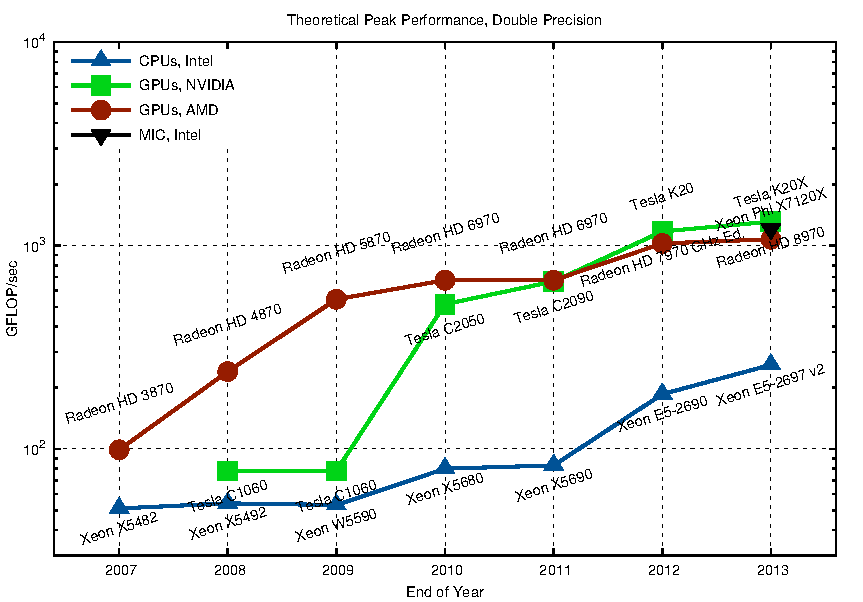
\includegraphics[width=0.95\textwidth]{figures/gflops-dp} \end{center}
\end{frame}

\begin{frame}{Hardware Specifications}
 \begin{block}{Peak Memory Bandwidth} \end{block}
 \begin{center} \vspace*{-0.9cm} 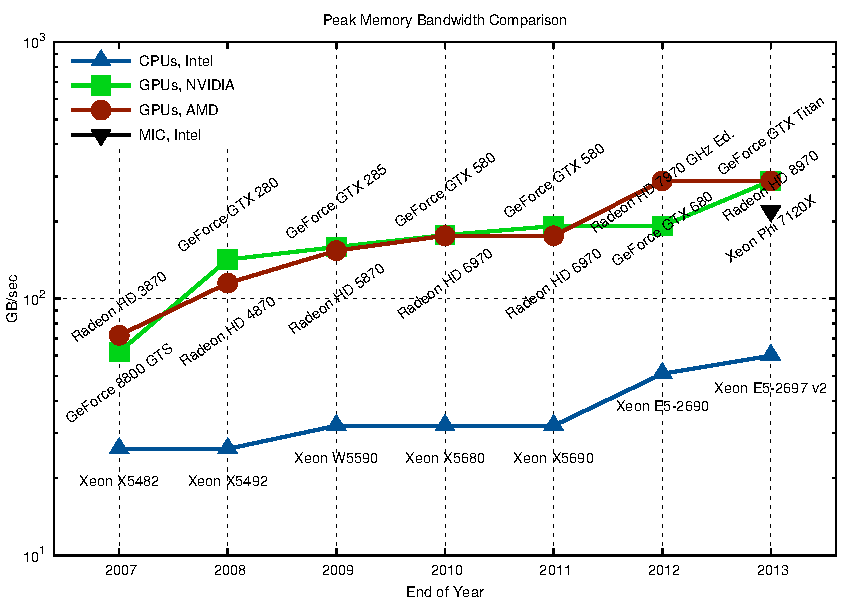
\includegraphics[width=0.95\textwidth]{figures/mem-bw} \end{center}
\end{frame}

\begin{frame}{Hardware Specifications}
 \begin{block}{FLOPs/Byte} \end{block}
 \begin{center} \vspace*{-0.9cm} 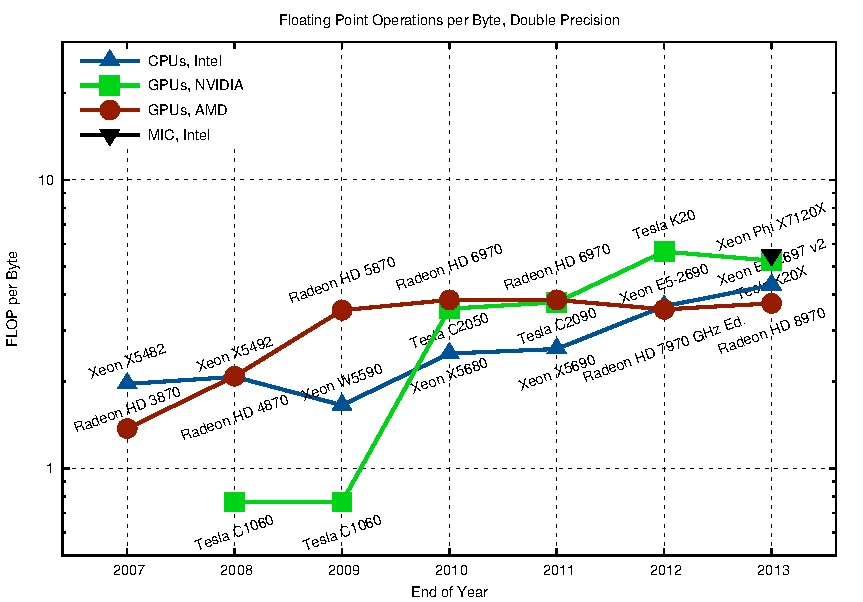
\includegraphics[width=0.95\textwidth]{figures/flop-per-byte-dp} \end{center}
\end{frame}

\begin{frame}{GPUs: Disillusion}
 \begin{center} 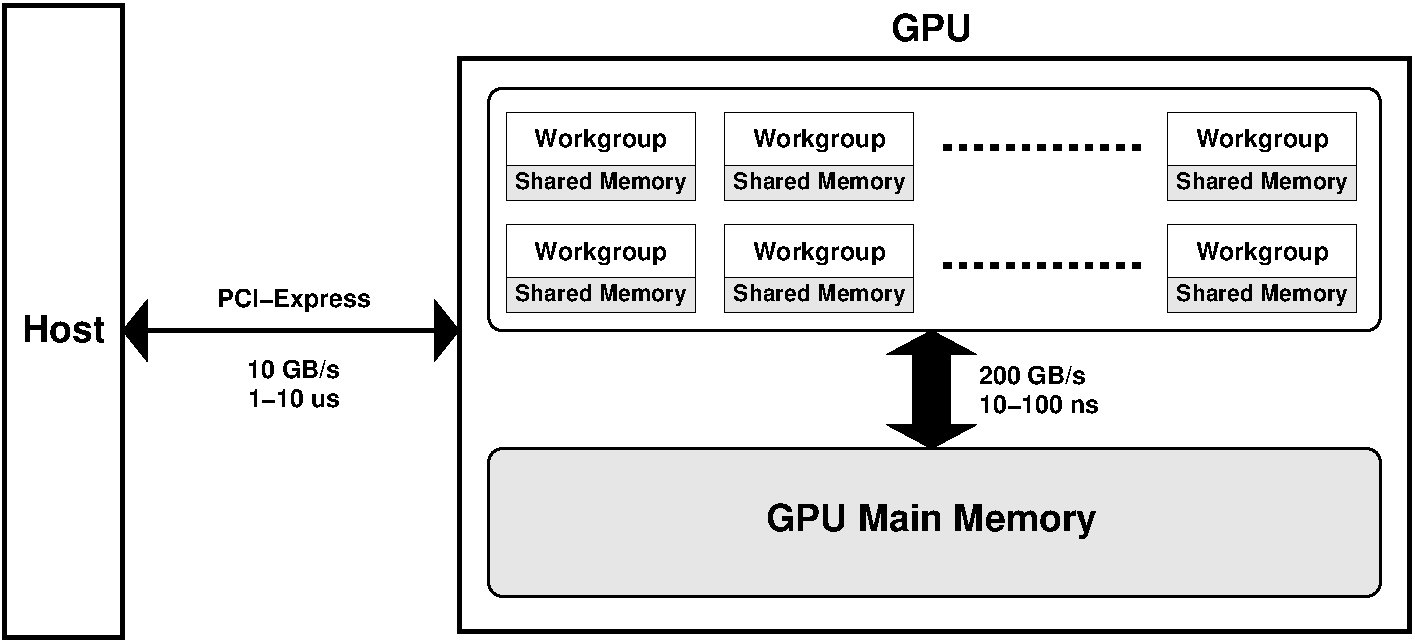
\includegraphics[width=0.99\textwidth]{figures/gpu-schematic} \end{center}
\end{frame}




%% About OpenCL
\begin{frame}{Table of Contents}
 \begin{block}{100x Speedup!?} \end{block}
 \begin{block}{\textbf{About OpenCL}} \end{block}
 \begin{block}{OpenCL Execution Model} \end{block}
 \begin{block}{OpenCL Kernel Language} \end{block}
 \begin{block}{Comparison with CUDA and OpenACC} \end{block}
 \begin{block}{Portable Performance} \end{block}
 \begin{block}{Summary} \end{block}
\end{frame}




\begin{frame}{History of OpenCL}

\begin{minipage}{0.7\textwidth}
\begin{block}{Prior to 2008}
  \begin{itemize}
   \item OpenCL developed by Apple Inc.
  \end{itemize}
\end{block}

\begin{block}{2008}
  \begin{itemize}
   \item OpenCL working group formed at Khronos Group
   \item OpenCL specification 1.0 released
  \end{itemize}
\end{block}

\begin{block}{2010}
  \begin{itemize}
   \item OpenCL 1.1 (multi-device, subbuffer manipulation)
  \end{itemize}
\end{block}

\begin{block}{2011}
  \begin{itemize}
   \item OpenCL 1.2 (device partitioning)
  \end{itemize}
\end{block}

\begin{block}{2013}
  \begin{itemize}
   \item OpenCL 2.0 (shared virtual memory, SPIR, etc.)
  \end{itemize}
\end{block}

\end{minipage} \hfill
\begin{minipage}{0.25\textwidth}
 
\includegraphics[width=0.99\textwidth]{figures/opencl.jpg}
 
 \vspace*{5cm}
\end{minipage}


\end{frame}





\begin{frame}{About OpenCL}

\begin{block}{Advantages}
  \begin{itemize}
   \item Not restricted to a single vendor: Intel, NVIDIA, AMD, ...
   \item Just a shared C-library
   \item Does not rely on compiler magic
  \end{itemize}
\end{block}

\pause
\begin{block}{Disadvantages}
  \begin{itemize}
   \item Not restricted to a single vendor
   \item Boilerplate code required
   \item Portable performance?
  \end{itemize}
\end{block}

\end{frame}






%% OpenCL Execution Model
\begin{frame}{Table of Contents}
 \begin{block}{100x Speedup!?} \end{block}
 \begin{block}{About OpenCL} \end{block}
 \begin{block}{\textbf{OpenCL Execution Model}} \end{block}
 \begin{block}{OpenCL Kernel Language} \end{block}
 \begin{block}{Comparison with CUDA and OpenACC} \end{block}
 \begin{block}{Portable Performance} \end{block}
 \begin{block}{Summary} \end{block}
\end{frame}

%%%%%%%%%%%%%%%%%%%% Platform Model %%%%%%%%%%%%%%%%%%%%%%

% \begin{frame}{OpenCL Platform Model}
%  \begin{center}
%    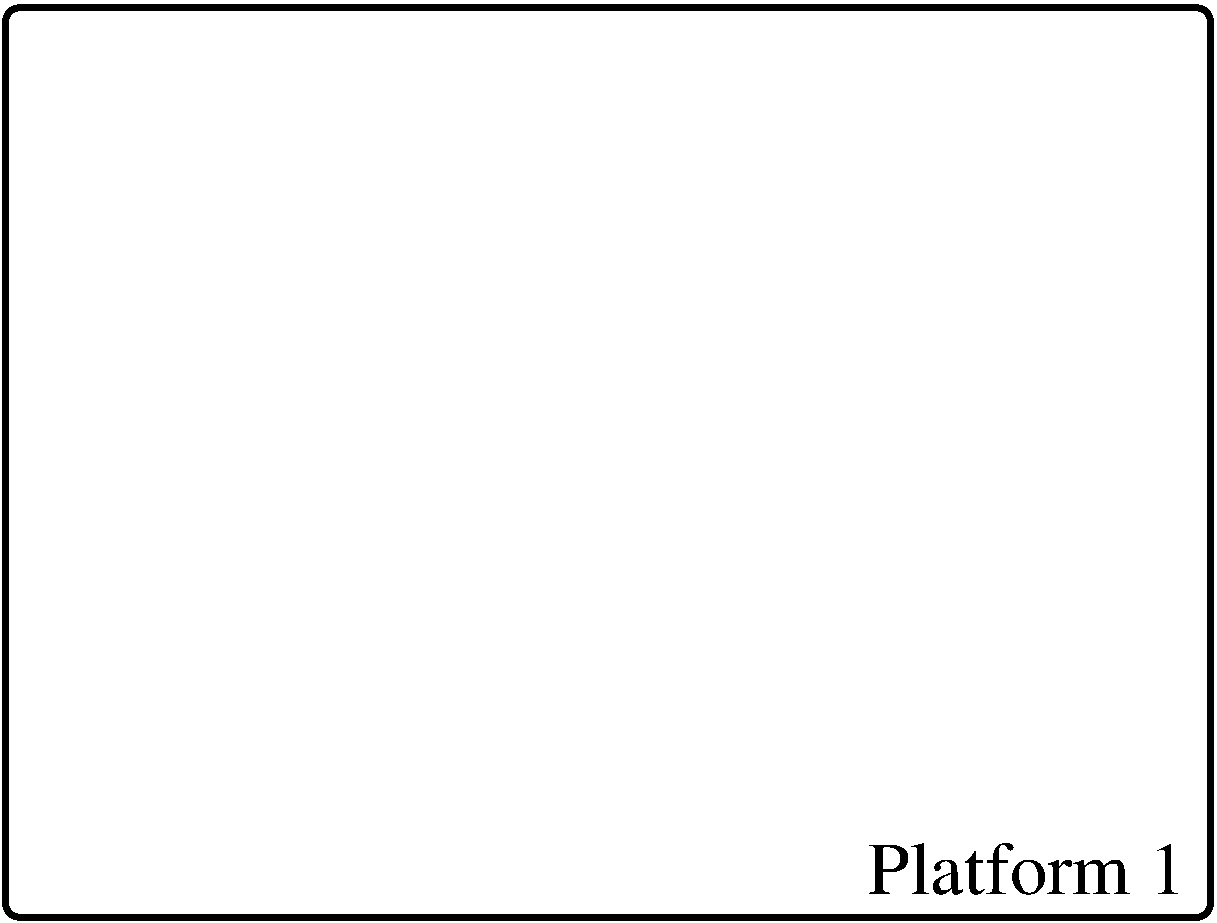
\includegraphics[width=0.80\textwidth]{figures/opencl-2.pdf}
%  \end{center}
% \end{frame}
% 
% \begin{frame}{OpenCL Platform Model}
%  \begin{center}
%    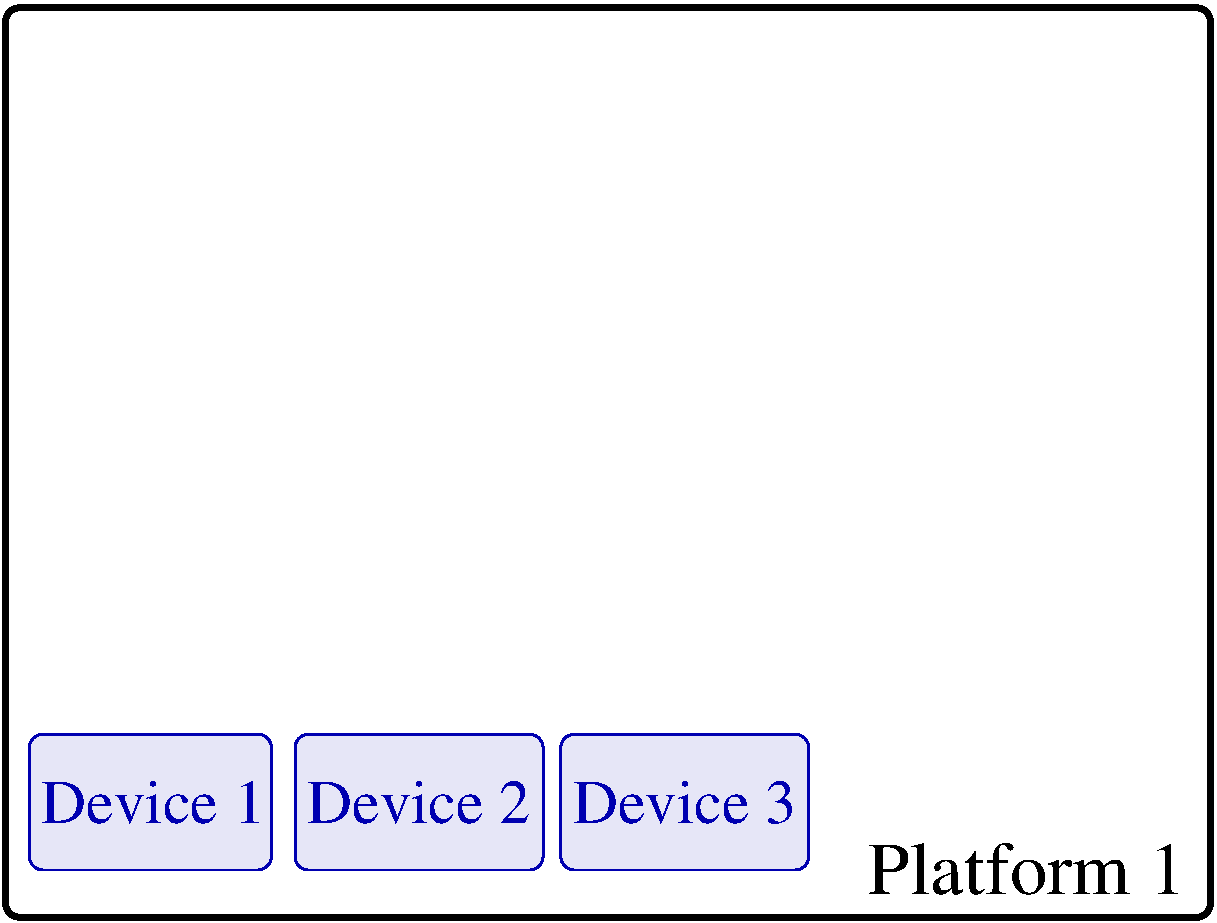
\includegraphics[width=0.80\textwidth]{figures/opencl-3.pdf}
%  \end{center}
% \end{frame}
% 
% \begin{frame}{OpenCL Platform Model}
%  \begin{center}
%    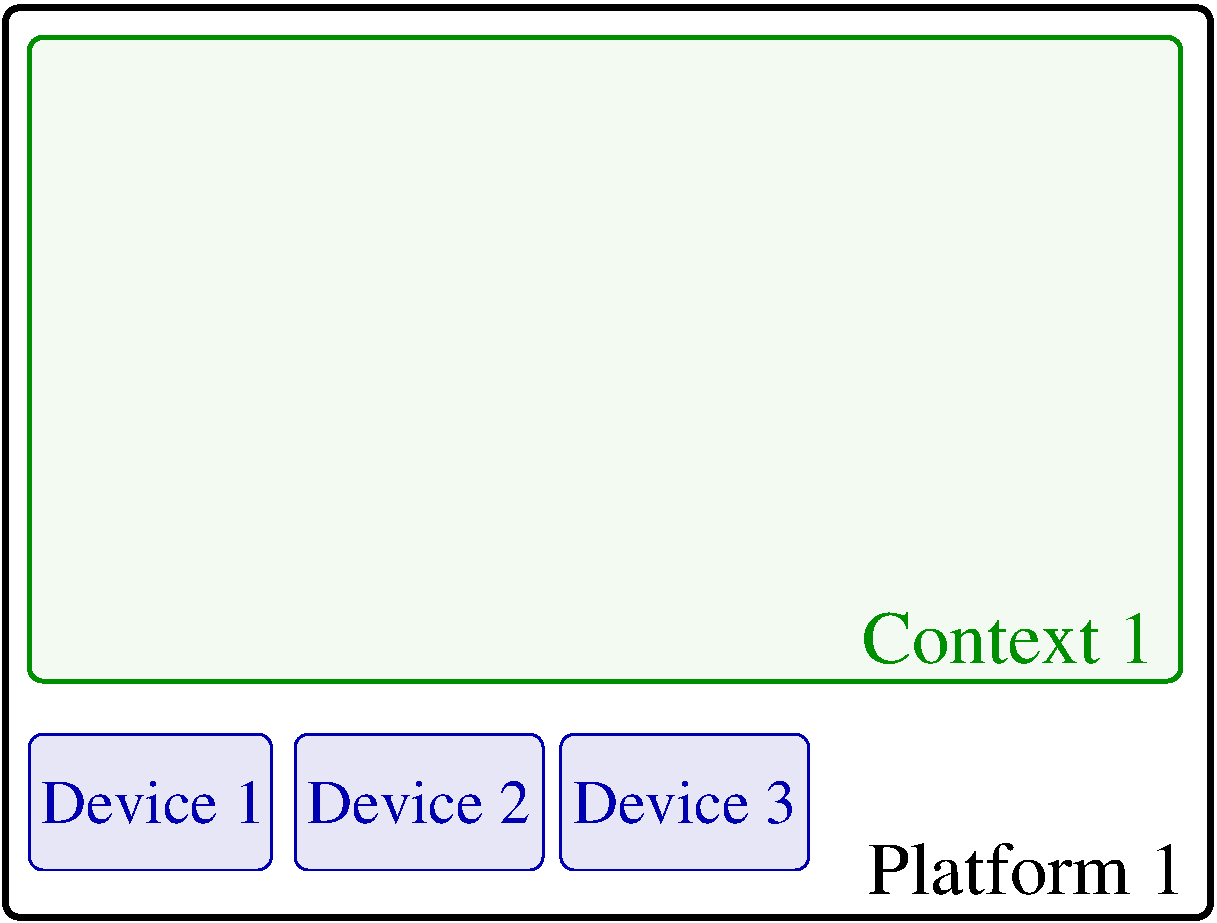
\includegraphics[width=0.80\textwidth]{figures/opencl-4.pdf}
%  \end{center}
% \end{frame}
% 
% \begin{frame}{OpenCL Platform Model}
%  \begin{center}
%    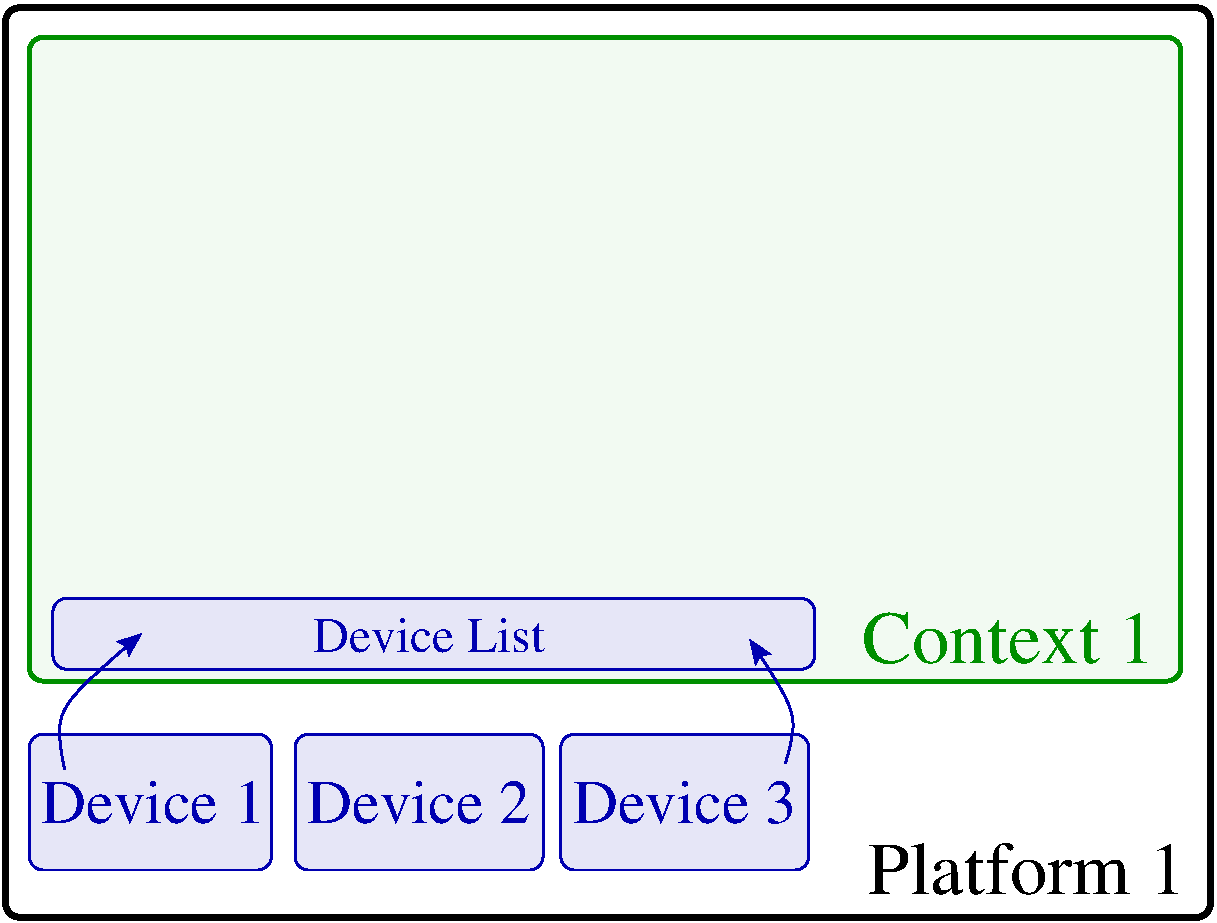
\includegraphics[width=0.80\textwidth]{figures/opencl-5.pdf}
%  \end{center}
% \end{frame}
% 
% \begin{frame}{OpenCL Platform Model}
%  \begin{center}
%    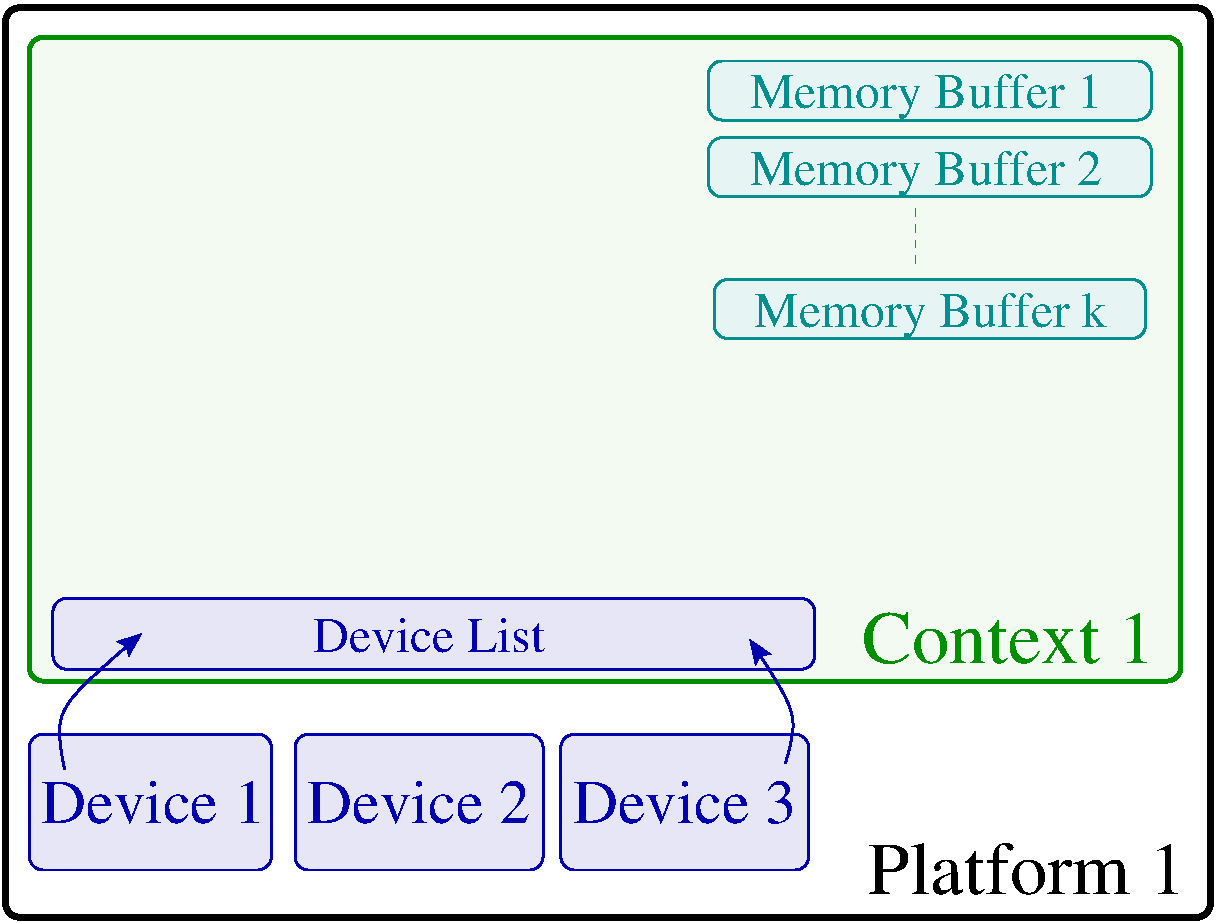
\includegraphics[width=0.80\textwidth]{figures/opencl-6.pdf}
%  \end{center}
% \end{frame}
% 
% \begin{frame}{OpenCL Platform Model}
%  \begin{center}
%    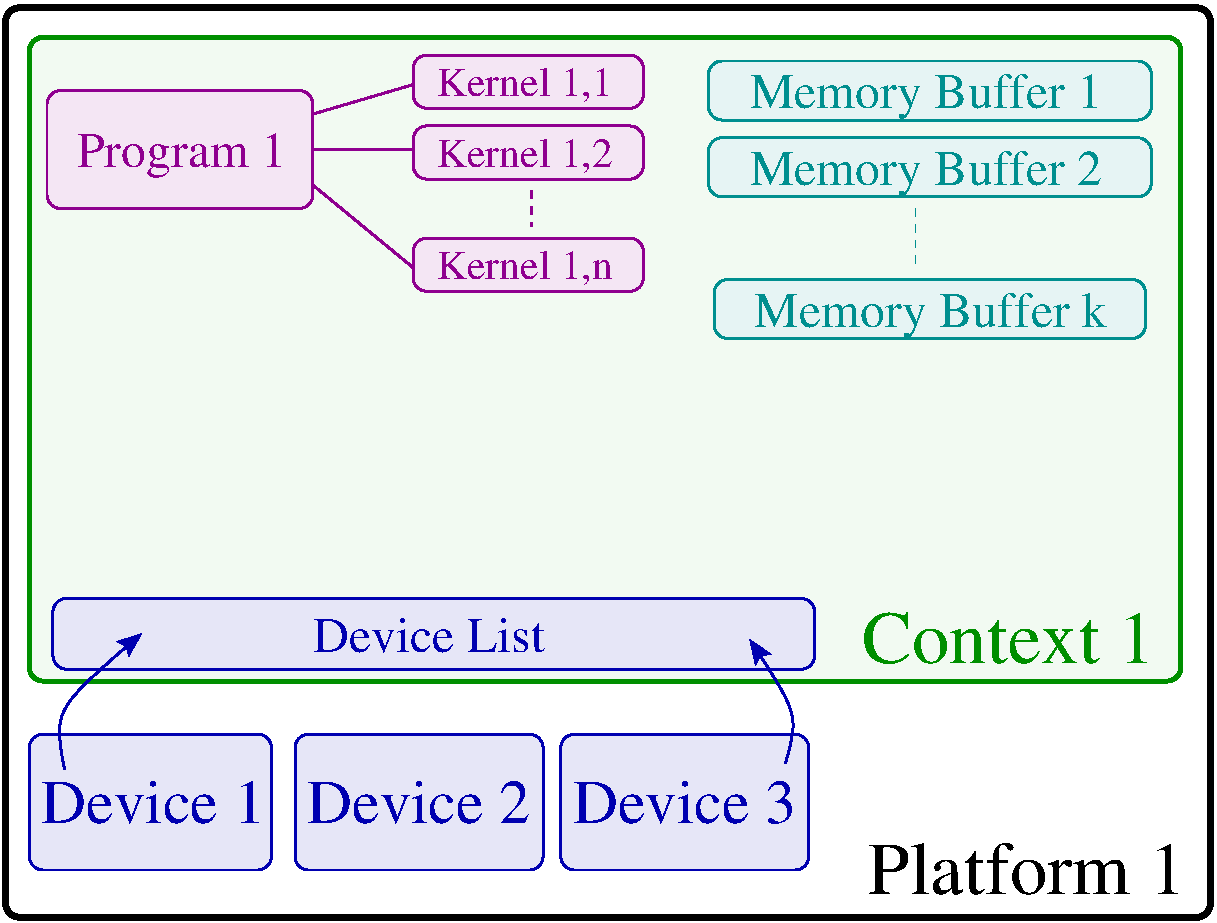
\includegraphics[width=0.80\textwidth]{figures/opencl-7.pdf}
%  \end{center}
% \end{frame}
% 
% \begin{frame}{OpenCL Platform Model}
%  \begin{center}
%    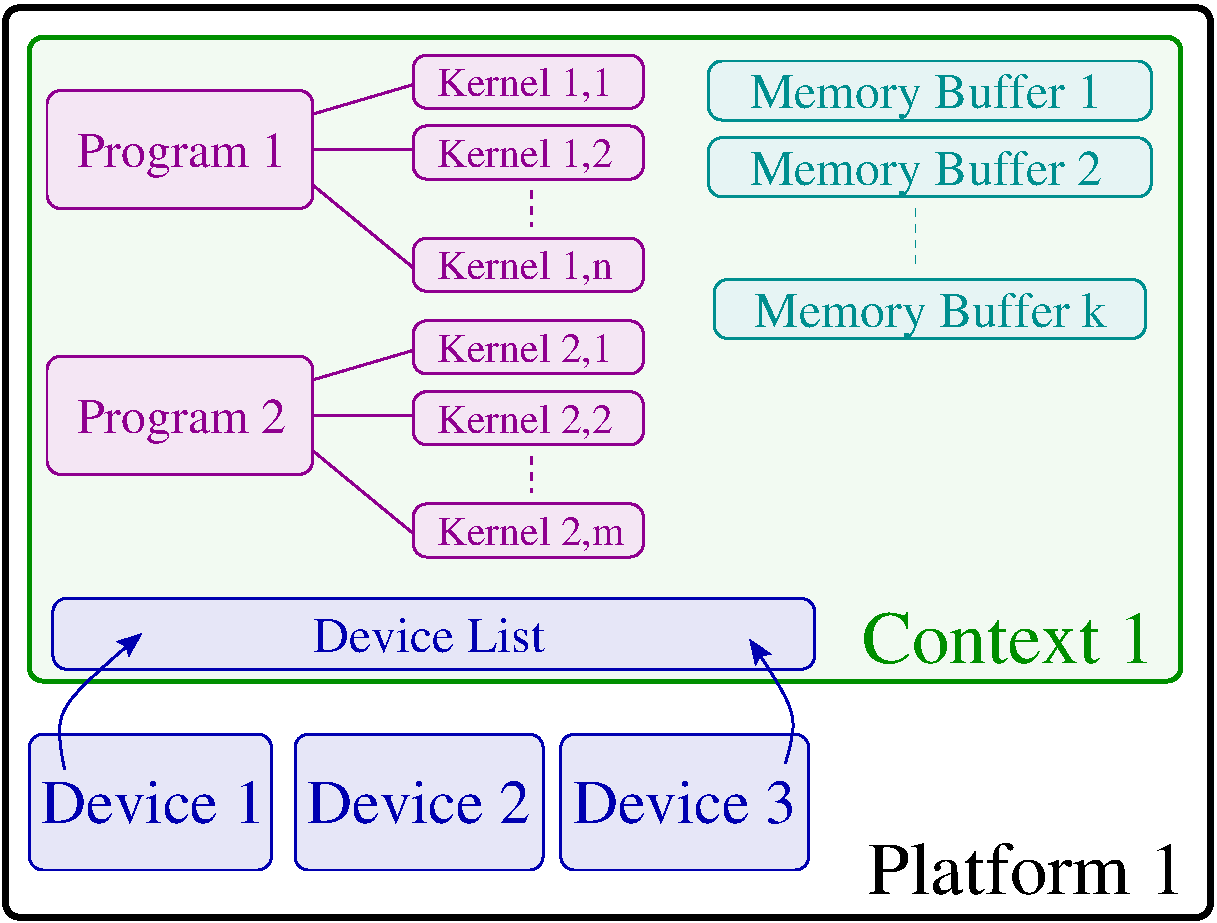
\includegraphics[width=0.80\textwidth]{figures/opencl-8.pdf}
%  \end{center}
% \end{frame}

\begin{frame}{OpenCL Platform Model}
 \begin{center}
   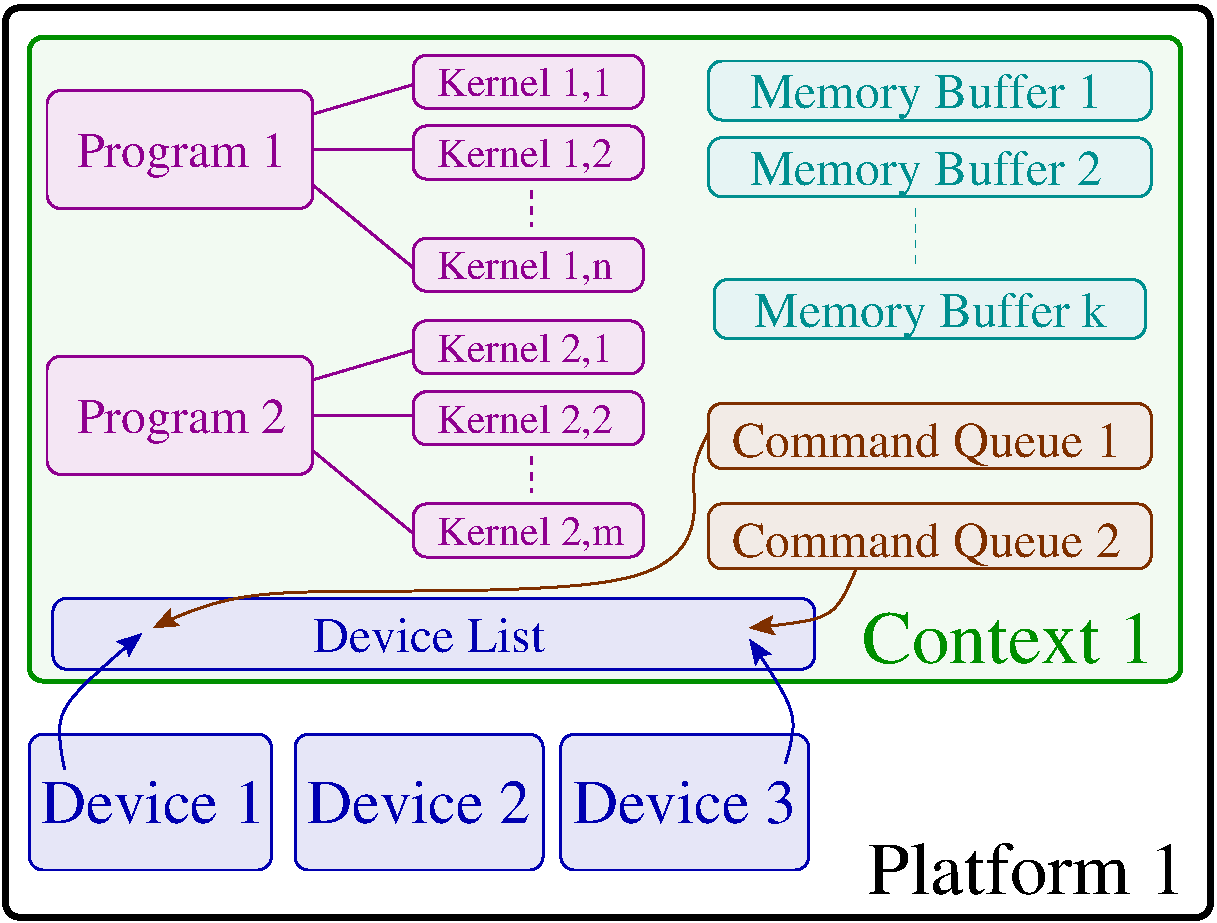
\includegraphics[width=0.80\textwidth]{figures/opencl-full.pdf}
 \end{center}
\end{frame}

\begin{frame}{OpenCL Platform Model}
 \begin{center}
   \Huge https://github.com/karlrupp/phsp2014
 \end{center}
\end{frame}





\begin{frame}[fragile]
\frametitle{OpenCL Host API}

\lstset{ basicstyle=\scriptsize\ttfamily }
\begin{lstlisting}[escapechar=@]
// Setup contet and queue
@\color{red}{context}@ = clCreateContextFromType(NULL, CL_DEVICE_TYPE_GPU, NULL, NULL, NULL);
@\color{red}{queue}@ = clCreateCommandQueue(context, NULL, 0, NULL);

// Create memory buffers
@\color{red}{memobjs[0]}@ = clCreateBuffer(context, CL_MEM_READ_WRITE, sizeof(float)*2*num_entries, NULL, NULL);
@\color{red}{memobjs[1]}@ = clCreateBuffer(context, CL_MEM_READ_ONLY | CL_MEM_COPY_HOST_PTR, sizeof(float)*2*num_entries, srcA, NULL);

// Create OpenCL program and kernels
@\color{red}{program}@ = clCreateProgramWithSource(context, 1, &kernel_src, NULL, NULL);
clBuildProgram(program, 0, NULL, NULL, NULL, NULL);
 
@\color{red}{kernel}@ = clCreateKernel(program, "my_kernel", NULL);
clSetKernelArg(kernel, 0, sizeof(cl_mem), (void *)&memobjs[0]);
clSetKernelArg(kernel, 1, sizeof(cl_mem), (void *)&memobjs[1]);
clSetKernelArg(kernel, 2, sizeof(float)*(local_work_size[0]+1)*16, NULL);
 
// Run an OpenCL kernel:
global_work_size[0] = 128;
 local_work_size[0] = 64;
clEnqueueNDRangeKernel(queue, kernel, 1, NULL, global_work_size, local_work_size, 0, NULL, NULL);
\end{lstlisting}
\lstset{ basicstyle=\small\ttfamily }

\begin{block}{Issues}
 \begin{itemize}
  \item ``Where is the error?''
  \item Manage OpenCL handles
 \end{itemize}

\end{block}

\end{frame}




%% OpenCL Kernel Language 
\begin{frame}{Table of Contents}
 \begin{block}{100x Speedup!?} \end{block}
 \begin{block}{About OpenCL} \end{block}
 \begin{block}{OpenCL Execution Model} \end{block}
 \begin{block}{\textbf{OpenCL Kernel Language}} \end{block}
 \begin{block}{Comparison with CUDA and OpenACC} \end{block}
 \begin{block}{Portable Performance} \end{block}
 \begin{block}{Summary} \end{block}
\end{frame}



\begin{frame}{OpenCL Kernel Language}

\begin{block}{Primer: OpenCL Device Execution Model}
 \begin{center}
   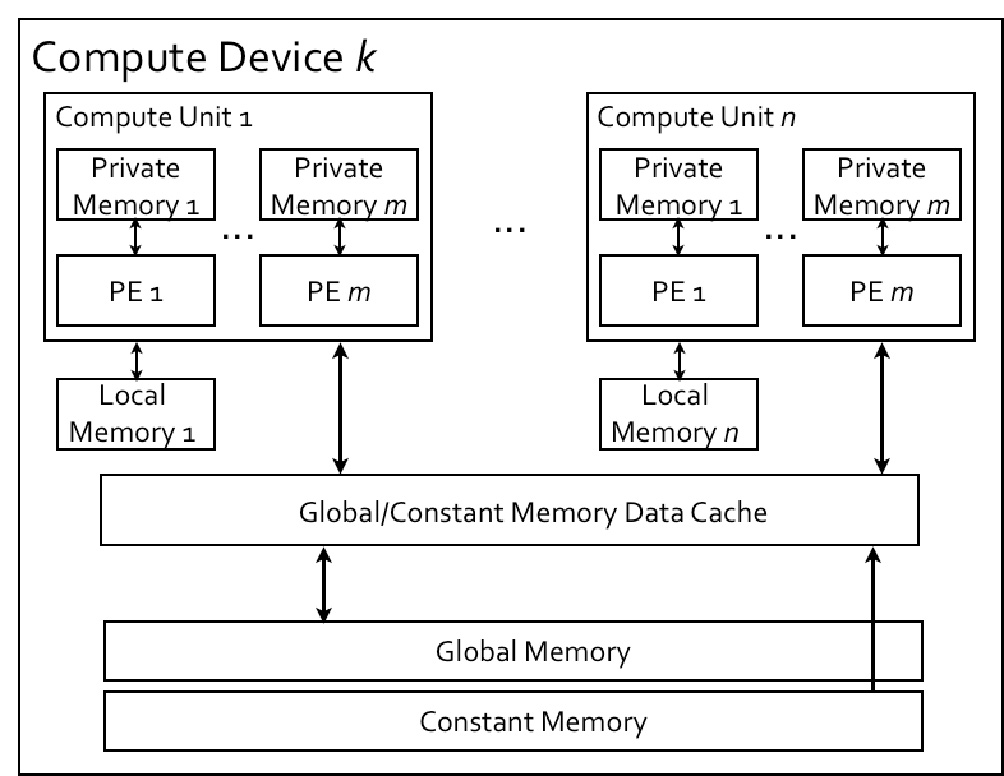
\includegraphics[width=0.73\textwidth]{figures/opencl-device.jpg} \\
 \end{center}
  {\tiny http://developer.amd.com/documentation/articles/PublishingImages/opencl\_figure5.jpg}
  \vspace{0.5cm}
\end{block}

\end{frame}




\begin{frame}[fragile]
\frametitle{OpenCL Kernel Language}

\begin{block}{Sample Operation: Inplace Vector Addition}
 \vspace*{-0.5cm}
 \begin{align*}
  \left(
  \begin{array}{c}
   x_1 \\
   x_2 \\
   \vdots \\
   x_n 
  \end{array} \right) +\!= 
  \left(
  \begin{array}{c}
   y_1 \\
   y_2 \\
   \vdots \\
   y_n 
  \end{array} \right)
 \end{align*}
\end{block}

 \vspace*{-0.3cm}
\begin{block}{OpenCL Kernel}
\begin{lstlisting}
__kernel void inplace_add(
          __global const float * vec1,
          __global const float * vec2,
          unsigned int size) 
{ 
  for (unsigned int i  = get_global_id(0); 
                    i  < size; 
                    i += get_global_size(0))
    x[i] += y[i];
}
\end{lstlisting}
\end{block}
\end{frame}




\begin{frame}[fragile]{OpenCL Kernel Language}

 \begin{block}{Just Like C}
  \begin{itemize}
   \item Datatypes: \lstinline|float|, \lstinline|double|, \lstinline|long|, ... , \lstinline|float2|, \lstinline|float4|, ...
   \item Keywords: \lstinline|for|, \lstinline|if|, \lstinline|switch|, ...
   \item ...
  \end{itemize}
 \end{block}

 \begin{block}{Thread Management}
  \begin{itemize}
   \item ID: \lstinline|get_local_id(dim)|, \lstinline|get_global_id(dim)|
   \item Count: \lstinline|get_local_size(dim)|, \lstinline|get_global_size(dim)|
   \item Sync: \lstinline|barrier(flags)|, \lstinline|mem_fence(flags)|
  \end{itemize}
 \end{block}

 \begin{block}{Memory Qualifiers}
  \begin{itemize}
   \item \lstinline|__global|: Global memory (e.g.~GPU RAM)
   \item \lstinline|__constant|: Constant global memory (vendor-specific!)
   \item \lstinline|__local|: Shared memory (per workgroup)
  \end{itemize}
 \end{block}

\end{frame}




\begin{frame}[fragile]{OpenCL Kernel Language}
  \begin{block}{Vector Assignment (Copy) Kernel}
    \begin{itemize}
     \item $x \Leftarrow y$ for (large) vectors $x$, $y$
    \end{itemize}
  \end{block}

  \only<1>{\vspace*{4.22cm}}
  \only<2>{\begin{center} \vspace*{0.84cm} 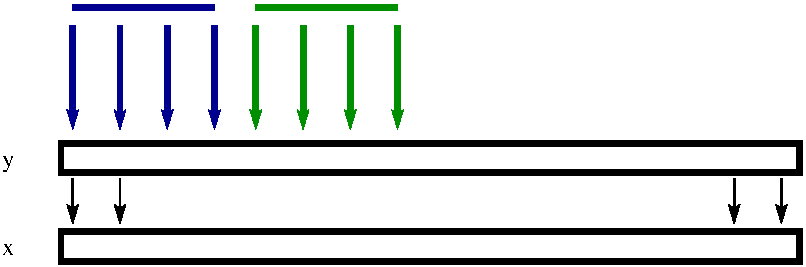
\includegraphics[width=0.8\textwidth]{figures/copy-kernel-gpu-1} \end{center}}
  \only<3>{\begin{center} \vspace*{0.85cm} 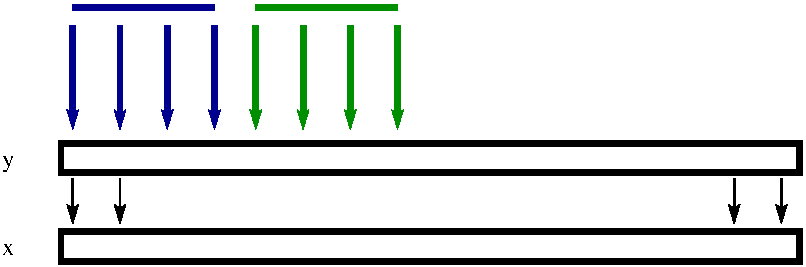
\includegraphics[width=0.8\textwidth]{figures/copy-kernel-gpu-1} \end{center}}
  \only<4>{\begin{center}                  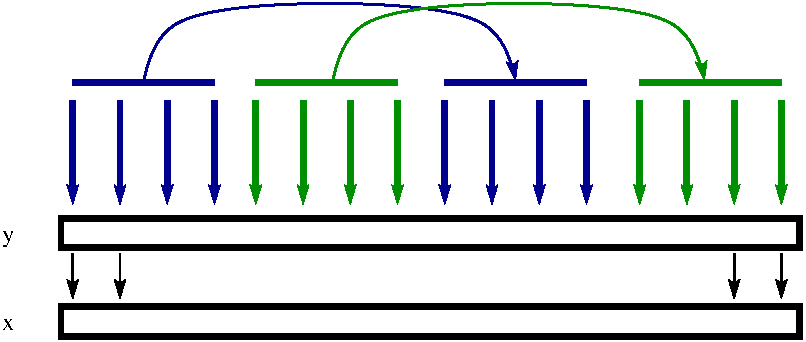
\includegraphics[width=0.8\textwidth]{figures/copy-kernel-gpu-full} \end{center}}
  
  \only<1>{\vspace*{2.52cm}}
  \only<2>{\vspace*{2.52cm}}
  \only<3>{
  \begin{block}{Parameters ($\gg 1000$ variations possible) }
   \begin{itemize}
    \item Local work size, global work size
    \item Vector types (float1, float2, ... , float16)
    \item Thread increment type
   \end{itemize}
  \end{block}}
  
  \only<4>{
  \begin{block}{Parameters ($\gg 1000$ variations possible) }
   \begin{itemize}
     \item \texttt{for (size\_t i = get\_global\_id(0); i < N;}
     \item \texttt{\ \ \ \ \ \ \ \ \ \ \ \ i+= get\_global\_size(0))}
     \item \texttt{\ \ x[i] = y[i];}
   \end{itemize}
  \end{block}
  }

\end{frame}


\begin{frame}{OpenCL Kernel Language}

  \begin{block}{No Synchronization: Vector Addition}
   \begin{center} 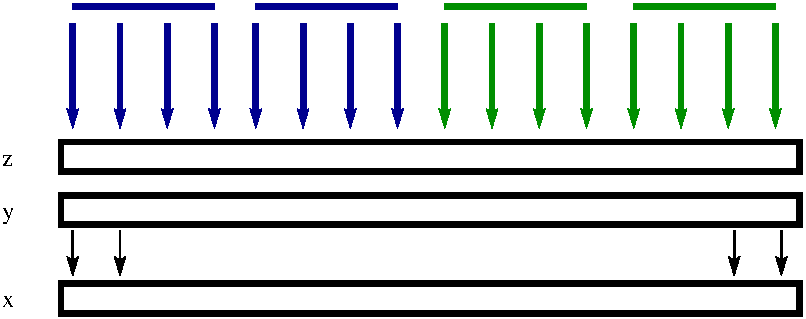
\includegraphics[width=0.6\textwidth]{figures/addition-kernel} \end{center}
  \end{block}
  
  \begin{block}{Synchronization: Dot Product}
   \begin{center} 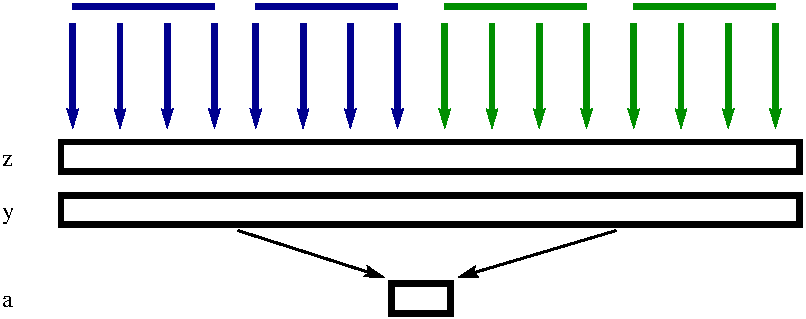
\includegraphics[width=0.6\textwidth]{figures/inner-product-kernel} \end{center}
  \end{block}

\end{frame}





%% Comparison with CUDA and OpenACC
\begin{frame}{Table of Contents}
 \begin{block}{100x Speedup!?} \end{block}
 \begin{block}{About OpenCL} \end{block}
 \begin{block}{OpenCL Execution Model} \end{block}
 \begin{block}{OpenCL Kernel Language} \end{block}
 \begin{block}{\textbf{Comparison with CUDA and OpenACC}} \end{block}
 \begin{block}{Portable Performance} \end{block}
 \begin{block}{Summary} \end{block}
\end{frame}





\begin{frame}[fragile]
\frametitle{Comparison with CUDA and OpenACC}
 \begin{block}{NVIDIA CUDA}
  \begin{lstlisting}
// GPU kernel:
__global__ void kernel(double *buffer)
{
  int idx = blockIdx.x * blockDim.x + threadIdx.x;
  buffer[idx] = 42.0;
}

// host code:
int main()
{ 
  ...
  cudaMalloc((void**)&buffer,size);
  kernel<<<blocknum, blockdim>>>(buffer);
  ...
}
  \end{lstlisting} 

  \begin{itemize}
   \item Almost no additional code required
   \item Vendor-lock
   \item Relies on \lstinline|nvcc| being available (plus version conflicts...)
  \end{itemize}
 \end{block}

\end{frame}



\begin{frame}[fragile]
\frametitle{Comparison with CUDA and OpenACC}
 \begin{block}{OpenCL}
  \begin{lstlisting}
const char *kernel_string =
"__kernel void mykernel(__global double *buffer) {
  buffer[get_global_id(0)] = 42.0;
};";   

int main() {
  ...
  cl_program my_prog = clCreateProgramWithSource(
         my_context,1,&kernel_string,&source_len,&err);
  clBuildProgram(my_prog,0,NULL,NULL,NULL,NULL);
  cl_kernel my_kernel = clCreateKernel(my_prog,
                          "mykernel",&err);
  clSetKernelArg(my_kernel,0,sizeof(cl_mem),&buffer);
  clEnqueueNDRangeKernel(queue,my_kernel,1,NULL,
               &global_size,&local_size,0,NULL,NULL);
} 
  \end{lstlisting} 

  \begin{itemize}
   \item Additional boilerplate code required (low-level API)
   \item Broad hardware support (separate SDKs)
   \item Second-best programming model for each vendor
  \end{itemize}
 \end{block}

\end{frame}






\begin{frame}[fragile]
\frametitle{Comparison with CUDA and OpenACC}
 \begin{block}{OpenACC}
  \begin{lstlisting}
void func(...) {
  #pragma acc data pcopyin(A[0:size][0:size])
  {
    #pragma acc kernels loop
    for(int i=0; i < size; i++)
      for(int j=0; j < size; j++)
        A[i][j] = 42;
  }
}

int main()
{
  double A[1337][1337];
  func(A);
}
  \end{lstlisting}

  \begin{itemize}
   \item Simple OpenMP-type pragma annotations
   \item Compiler support?
   \item Insufficient control over memory transfers?
  \end{itemize}
 \end{block}

\end{frame}




\begin{frame}[fragile]
\frametitle{Comparison with CUDA and OpenACC}
 \begin{block}{Thread Explosion Problem}
  \begin{lstlisting}
void func(double *A) {
  #pragma omp parallel for
  for(int i=0; i<1337; i++) A[i] = 42.0;
}

void func2(double *A) {
  #pragma omp parallel for
  for(int i=0; i<1337; i++) func(A);
}

int main() {
  double A[1337];
  func(A);  // okay
  func2(A); // boom...
}
  \end{lstlisting}

  \begin{itemize}
   \item Usually not as obvious as here
   \item Problem when OpenMP'ing MPI code
   \item Headache for library implementors
  \end{itemize}
 \end{block}

\end{frame}

% 
% \begin{frame}[fragile]
% \frametitle{GPUs: Library Aspects}
% 
%  \begin{block}{Challenge: Hardware}
%   \begin{itemize}
%    \item Portable performance
%    \item Auto-tuning
%    \item Testing requires many different machines
%   \end{itemize}
%  \end{block}
% 
%  \begin{block}{Challenge: Memory}
%   \begin{itemize}
%    \item Allocation failures?
%    \item Multi-GPU?
%    \item PCI-Express bottleneck
%   \end{itemize}
%  \end{block}
% 
%  \begin{block}{Challenge: Programming}
%   \begin{itemize}
%    \item Kernel language?
%    \item Which low-level parameters to expose?
%   \end{itemize}
%  \end{block}
% 
% \end{frame}
% 
% 



%% Portable Performance Section
\begin{frame}{Table of Contents}
 \begin{block}{100x Speedup!?} \end{block}
 \begin{block}{About OpenCL} \end{block}
 \begin{block}{OpenCL Execution Model} \end{block}
 \begin{block}{OpenCL Kernel Language} \end{block}
 \begin{block}{Comparison with CUDA and OpenACC} \end{block}
 \begin{block}{\textbf{Portable Performance}} \end{block}
 \begin{block}{Summary} \end{block}
\end{frame}





%\begin{frame}{Benchmarks}
%  \begin{center}
%   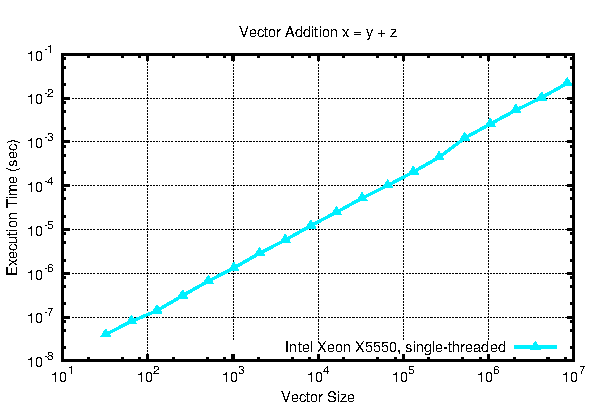
\includegraphics[width=0.95\textwidth]{figures/vector-timings-1}
%  \end{center}
%\end{frame}

%\begin{frame}{Benchmarks}
%  \begin{center}
%   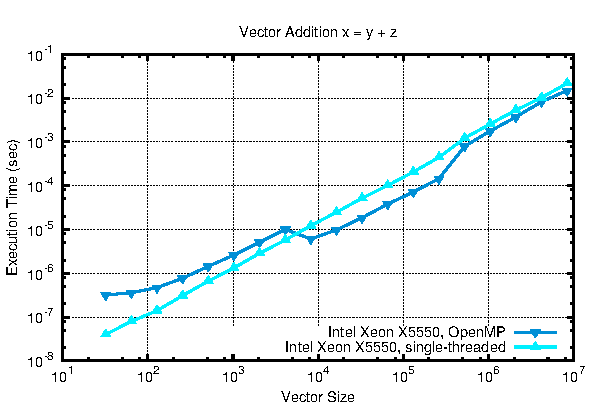
\includegraphics[width=0.95\textwidth]{figures/vector-timings-2}
%  \end{center}
%\end{frame}

%\begin{frame}{Benchmarks}
%  \begin{center}
%   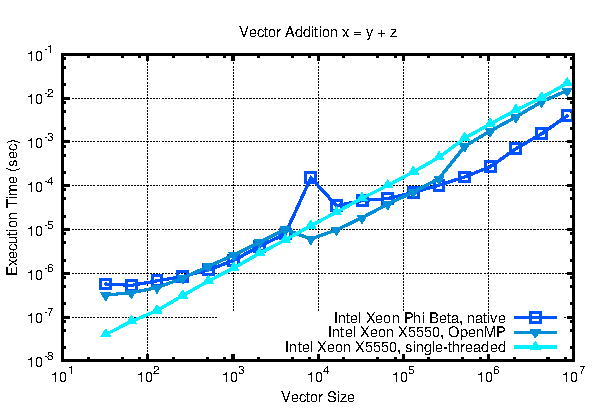
\includegraphics[width=0.95\textwidth]{figures/vector-timings-3}
%  \end{center}
%\end{frame}

%\begin{frame}{Benchmarks}
%  \begin{center}
%   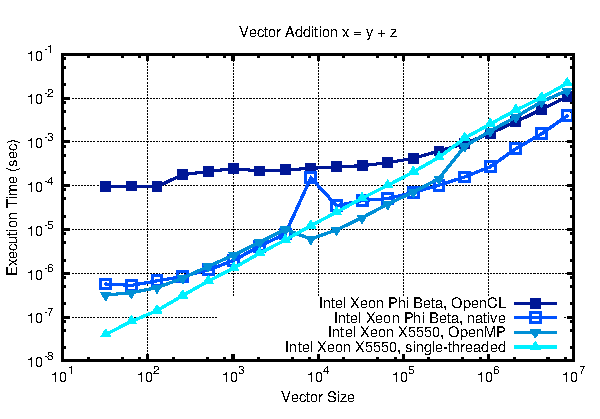
\includegraphics[width=0.95\textwidth]{figures/vector-timings-4}
%  \end{center}
%\end{frame}

%\begin{frame}{Benchmarks}
%  \begin{center}
%   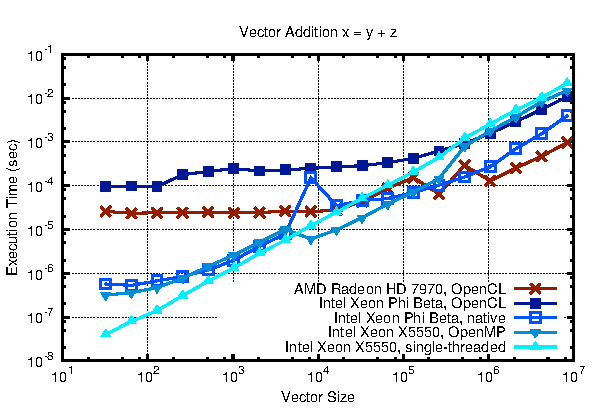
\includegraphics[width=0.95\textwidth]{figures/vector-timings-5}
%  \end{center}
%\end{frame}

%\begin{frame}{Benchmarks}
%  \begin{center}
%   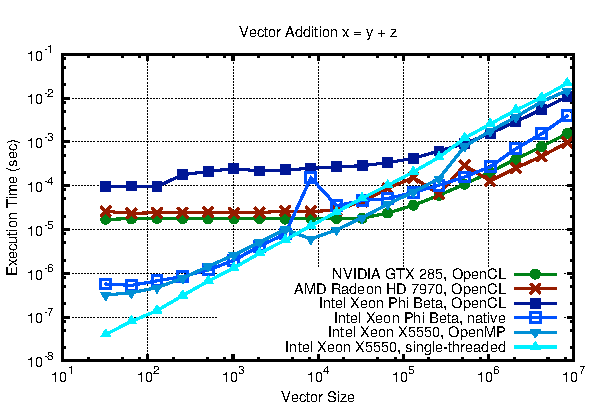
\includegraphics[width=0.95\textwidth]{figures/vector-timings-6}
%  \end{center}
%\end{frame}

\begin{frame}{Benchmarks}
  \begin{center}
   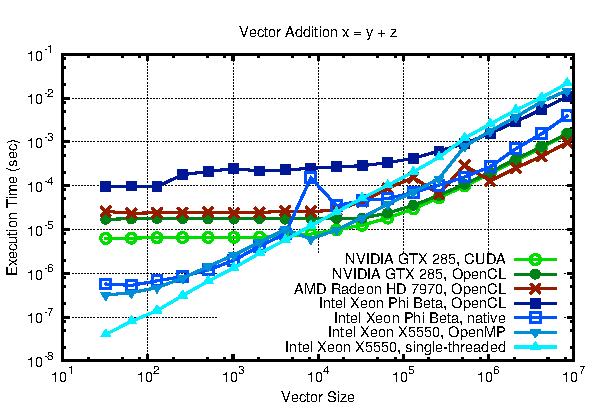
\includegraphics[width=0.95\textwidth]{figures/vector-timings-7}
  \end{center}
\end{frame}

%%

%\begin{frame}{Benchmarks}
%  \begin{center}
%   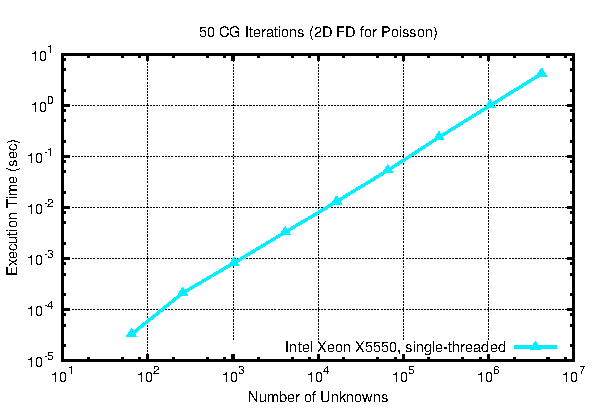
\includegraphics[width=0.95\textwidth]{figures/cg-timings-1}
%  \end{center}
%\end{frame}

%\begin{frame}{Benchmarks}
%  \begin{center}
%   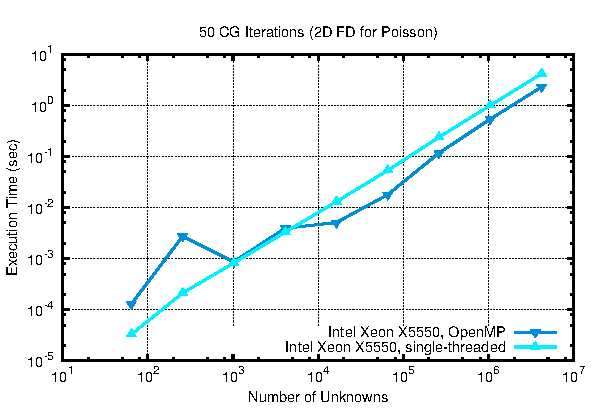
\includegraphics[width=0.95\textwidth]{figures/cg-timings-2}
%  \end{center}
%\end{frame}

%\begin{frame}{Benchmarks}
%  \begin{center}
%   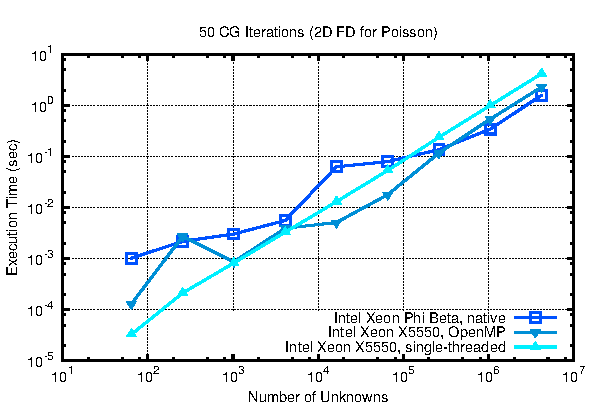
\includegraphics[width=0.95\textwidth]{figures/cg-timings-3}
%  \end{center}
%\end{frame}

%\begin{frame}{Benchmarks}
%  \begin{center}
%   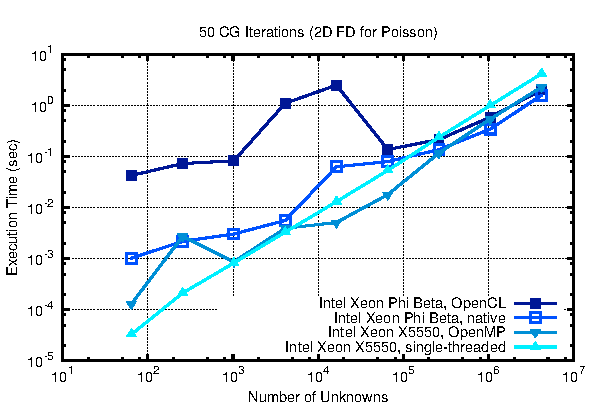
\includegraphics[width=0.95\textwidth]{figures/cg-timings-4}
%  \end{center}
%\end{frame}

%\begin{frame}{Benchmarks}
%  \begin{center}
%   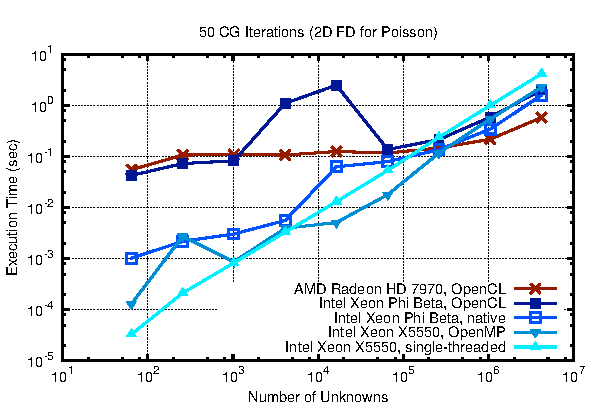
\includegraphics[width=0.95\textwidth]{figures/cg-timings-5}
%  \end{center}
%\end{frame}

%\begin{frame}{Benchmarks}
%  \begin{center}
%   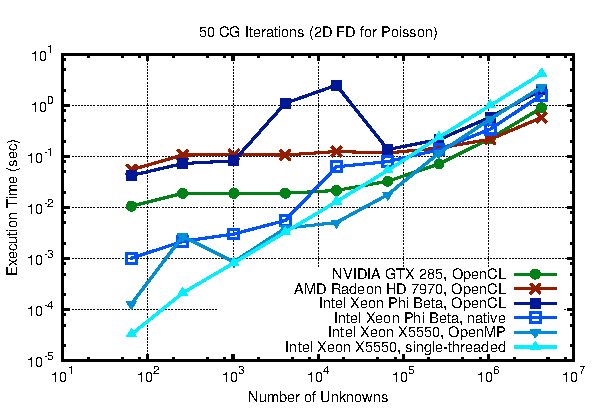
\includegraphics[width=0.95\textwidth]{figures/cg-timings-6}
%  \end{center}
%\end{frame}

\begin{frame}{Benchmarks}
  \begin{center}
   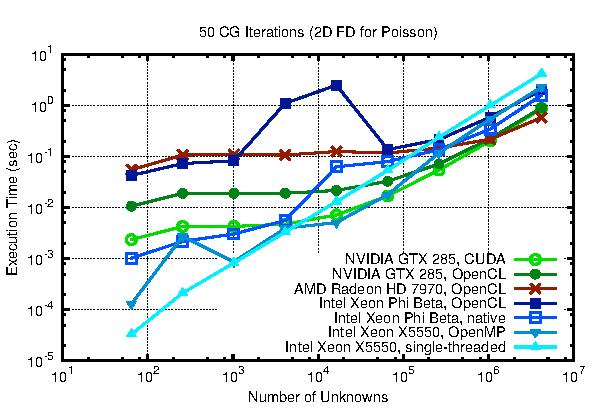
\includegraphics[width=0.95\textwidth]{figures/cg-timings-7}
  \end{center}
\end{frame}


\begin{frame}{Benchmarks}

 \begin{block}{Matrix-Matrix Multiplication}
  \begin{itemize}
   \item Autotuning environment 
   \item 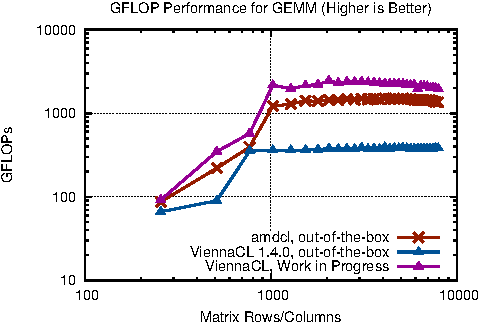
\includegraphics[width=0.85\textwidth]{figures/gemm3.pdf}
   \item \centering (AMD Radeon HD 7970, single precision)
  \end{itemize}

 \end{block}

\end{frame}






\begin{frame}{Benchmark Setting}

  \begin{block}{Scope for OpenCL-based Portability Study}
    \begin{itemize}
     \item Vector and matrix-vector operations (BLAS levels 1 and 2)
     \item Limited by memory bandwidth
     %\item Matrix-matrix-multiplication (only briefly today)
    \end{itemize}
  \end{block}

  \pause
  \begin{block}{Key Question (Memory-Bandwidth-Limited Kernels)}
    \begin{center} \color{red} \LARGE
     Good performance of complicated kernels \\
     by optimizing the simplest kernel?
    \end{center}
  \end{block}

\end{frame}


%% Copy kernel:
\begin{frame}[fragile]{Benchmark Setting}
  \begin{block}{Vector Assignment (Copy) Kernel}
    \begin{itemize}
     \item $x \Leftarrow y$ for (large) vectors $x$, $y$
    \end{itemize}
  \end{block}

  \only<1>{\begin{center} \vspace*{0.85cm} 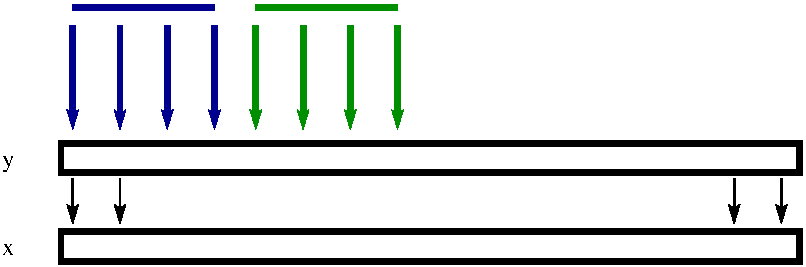
\includegraphics[width=0.8\textwidth]{figures/copy-kernel-gpu-1} \end{center}}
  \only<2>{\begin{center}                  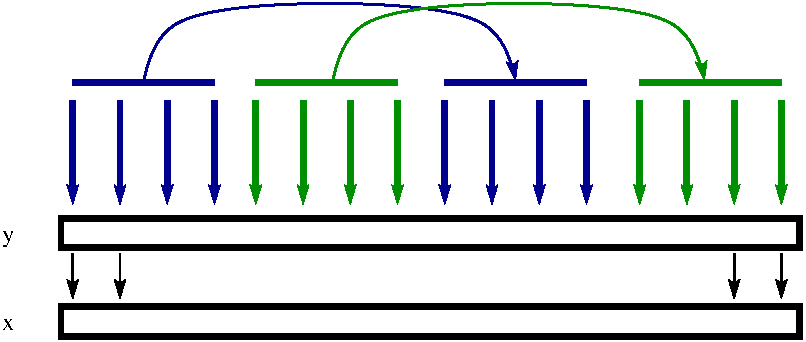
\includegraphics[width=0.8\textwidth]{figures/copy-kernel-gpu-full} \end{center}}
  \only<3>{\begin{center} \vspace*{0.84cm} 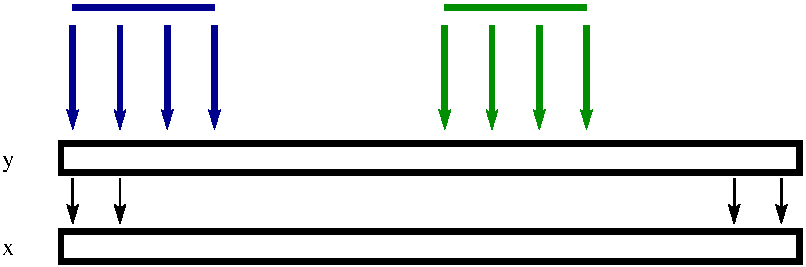
\includegraphics[width=0.8\textwidth]{figures/copy-kernel-cpu-1} \end{center}}
  \only<4>{\begin{center} \vspace*{0.30cm} 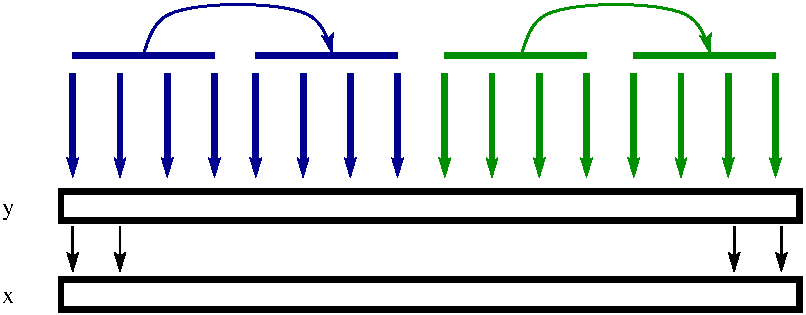
\includegraphics[width=0.8\textwidth]{figures/copy-kernel-cpu-full} \end{center}}
  
  \only<1>{
  \begin{block}{Parameters (1900 variations) }
   \begin{itemize}
    \item Local work size, global work size
    \item Vector types (float1, float2, ... , float16)
    \item Thread increment type
   \end{itemize}
  \end{block}}
  
  \only<2>{
  \begin{block}{Parameters (1900 variations) }
   \begin{itemize}
     \item \texttt{for (size\_t i = get\_global\_id(0); i < N;}
     \item \texttt{\ \ \ \ \ \ \ \ \ \ \ \ i+= get\_global\_size(0))}
     \item \texttt{\ \ x[i] = y[i];}
   \end{itemize}
  \end{block}
  }

  \only<3>{
  \begin{block}{Parameters (1900 variations) }
   \begin{itemize}
     \item \texttt{for (size\_t i = group\_start + get\_local\_id(0);}
     \item \texttt{\ \ \ \ \ i < group\_end; i+= get\_local\_size(0)) }
     \item \texttt{\ \  x[i] = y[i];}
   \end{itemize}
  \end{block}
  }

  \only<4>{
  \begin{block}{Parameters (1900 variations) }
   \begin{itemize}
     \item \texttt{for (size\_t i = group\_start + get\_local\_id(0);}
     \item \texttt{\ \ \ \ \ i < group\_end; i+= get\_local\_size(0)) }
     \item \texttt{\ \  x[i] = y[i];}
   \end{itemize}
  \end{block}
  }
\end{frame}


%% 
\begin{frame}{Benchmark Setting}

  \begin{block}{Operations}
   \begin{itemize}
    \item Vector copy, vector addition, inner product
    \item Matrix-vector product
   \end{itemize}
  \end{block}

  %\only<1>{\begin{center} 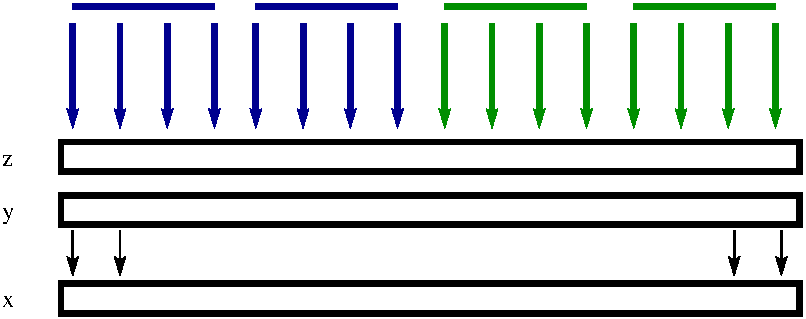
\includegraphics[width=0.8\textwidth]{figures/addition-kernel} \end{center}}
  %\only<2>{\begin{center} 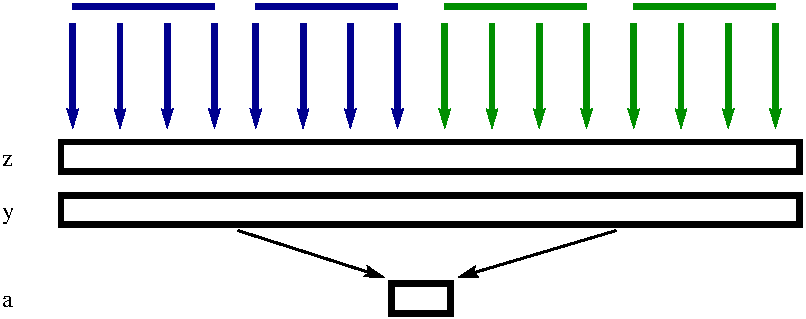
\includegraphics[width=0.8\textwidth]{figures/inner-product-kernel} \end{center}}

  %\visible<3->{
  \begin{center} 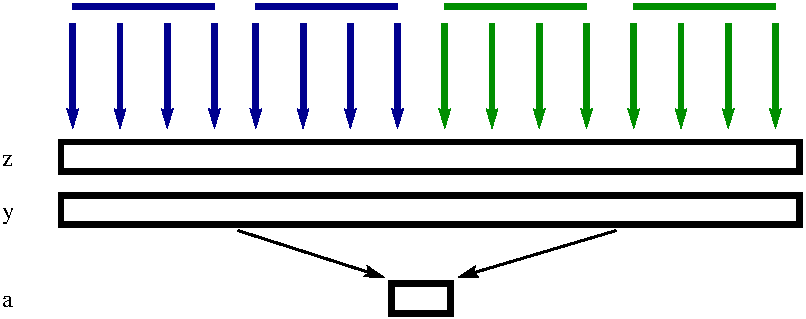
\includegraphics[width=0.8\textwidth]{figures/inner-product-kernel} \end{center}

  \begin{block}{Devices}
   \begin{itemize}
    \item AMD: A10-5800 APU, HD 5850 GPU
    \item INTEL: Dual Socket Xeon E5-2670, Xeon Phi
    \item NVIDIA: GTX 285, Tesla K20m
   \end{itemize}
  \end{block}
  %}
  
\end{frame}



\begin{frame}{Portable Performance}
  \begin{center} \Large \textbf{Histograms} \end{center}
\end{frame}

\begin{frame}{Portable Performance}
  \begin{center} 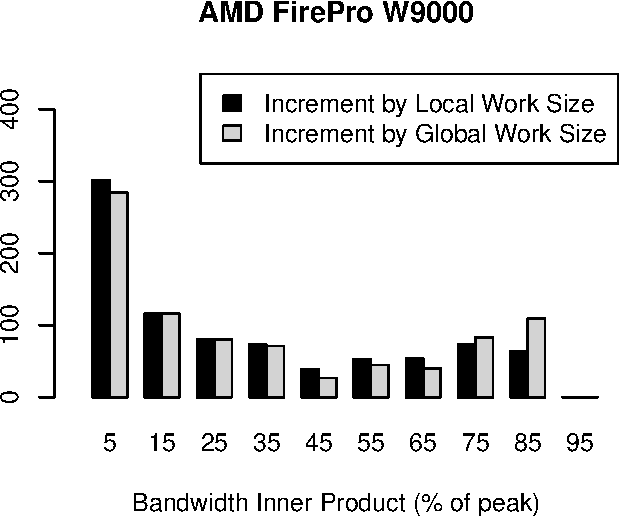
\includegraphics[width=0.75\textwidth]{figures/firepro_w9000_double_hist_itertype_dot} \end{center}
\end{frame}

\begin{frame}{Portable Performance}
  \begin{center} 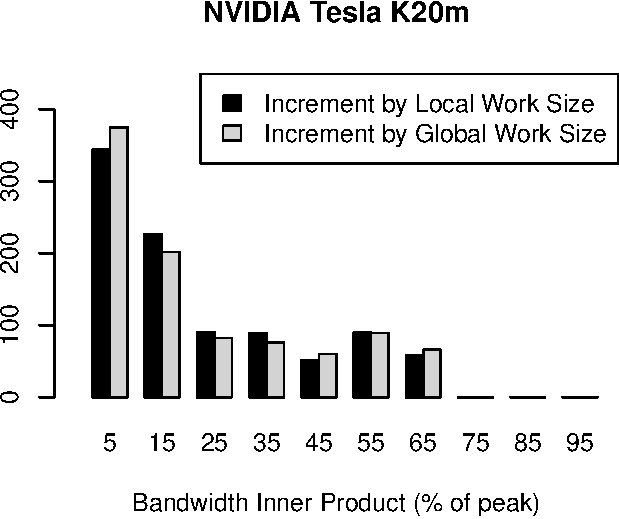
\includegraphics[width=0.75\textwidth]{figures/k20m_double_hist_itertype_dot} \end{center}
\end{frame}

\begin{frame}{Portable Performance}
  \begin{center} 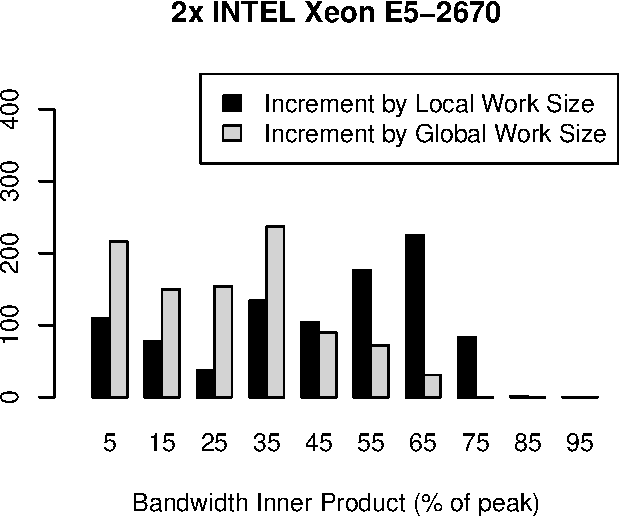
\includegraphics[width=0.75\textwidth]{figures/xeon_cpu_double_hist_itertype_dot} \end{center}
\end{frame}

\begin{frame}{Portable Performance}
  \begin{center} 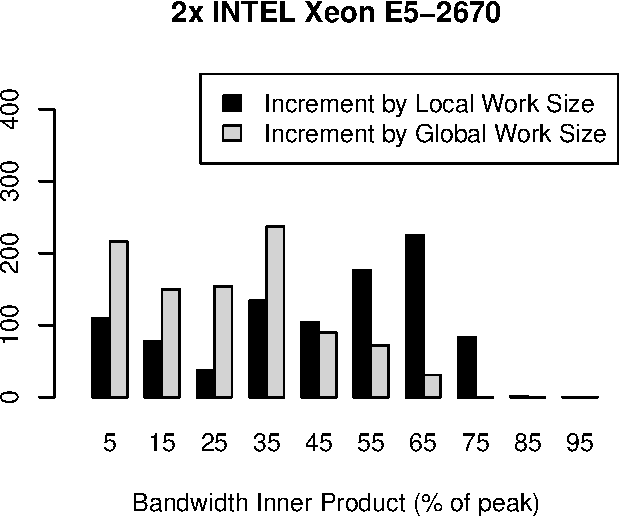
\includegraphics[width=0.55\textwidth]{figures/xeon_cpu_double_hist_itertype_dot} \\[1em]
                 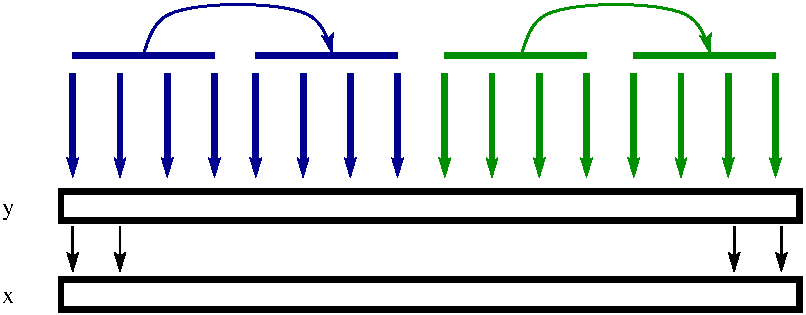
\includegraphics[width=0.45\textwidth]{figures/copy-kernel-cpu-full} 
  \end{center}
\end{frame}


%%%%%%%%%%%%%%%%%%%%%%%%%%%%%%%%%%%%%%%%%%%%%%%%%%%%%%%%%%%%%%%


\begin{frame}{Portable Performance}
  \begin{center} \textbf{ [Addition$|$Inner Product$|$Matrix-Vector] vs. Copy Kernel }\\[1em] Same Device \end{center}
\end{frame}

\begin{frame}{Portable Performance}
  \only<1>{\begin{center} 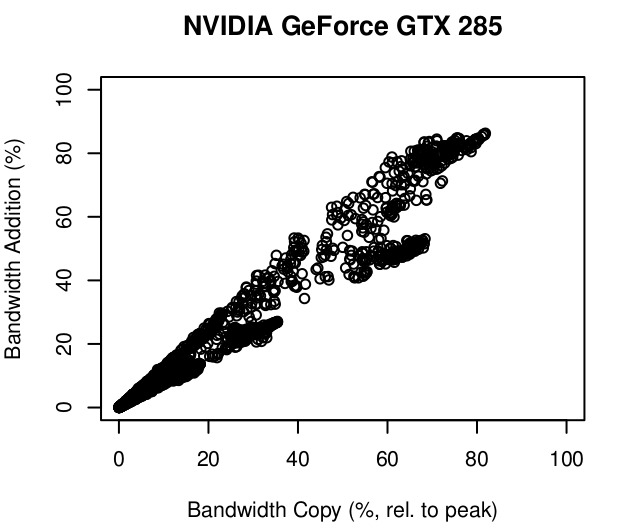
\includegraphics[width=0.8\textwidth]{figures/gtx285-addition-copy-1} \end{center}}
  \only<2>{\begin{center} 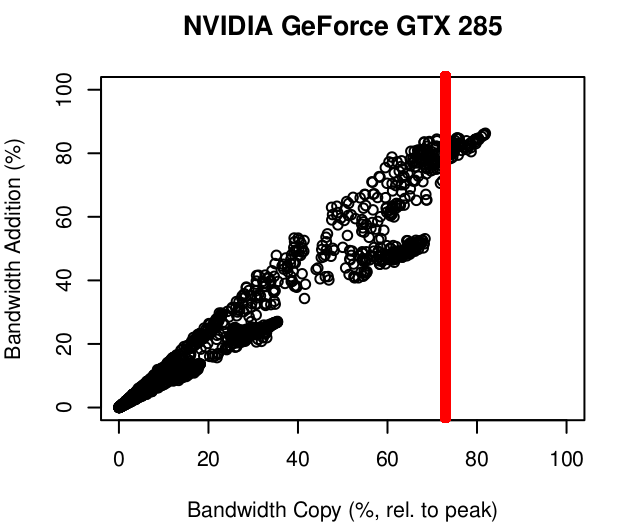
\includegraphics[width=0.8\textwidth]{figures/gtx285-addition-copy-2} \end{center}}
  \only<3>{\begin{center} 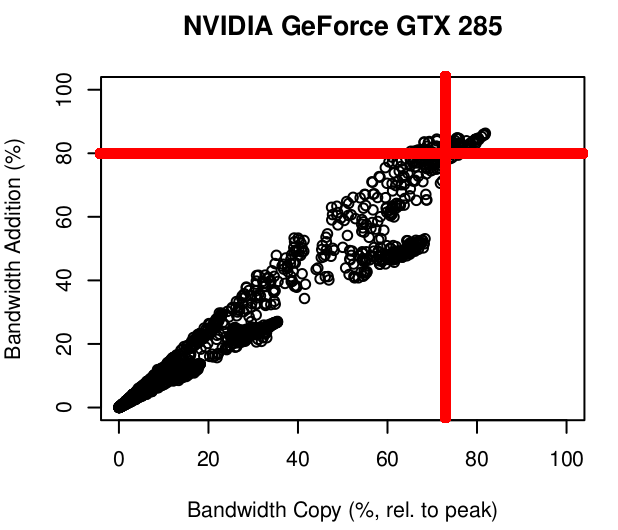
\includegraphics[width=0.8\textwidth]{figures/gtx285-addition-copy-3} \end{center}}
\end{frame}


\begin{frame}{Portable Performance}
  \only<1>{\begin{center} {\LARGE NVIDIA Tesla K20m} \\[2em]       \hspace*{1.cm} Addition \hspace*{2.1cm} Inner Product \hspace*{1.4cm} Mat-Vec Product \\[1em] \includegraphics[width=0.99\textwidth]{figures/k20m_double_xy_copy-crop} \end{center}}
  \only<2>{\begin{center} {\LARGE AMD Radeon HD 5850} \\[2em]      \hspace*{1.cm} Addition \hspace*{2.1cm} Inner Product \hspace*{1.4cm} Mat-Vec Product \\[1em] \includegraphics[width=0.99\textwidth]{figures/hd5850_double_xy_copy-crop} \end{center}}
  \only<3>{\begin{center} {\LARGE AMD FirePro W9000} \\[2em]       \hspace*{1.cm} Addition \hspace*{2.1cm} Inner Product \hspace*{1.4cm} Mat-Vec Product \\[1em] \includegraphics[width=0.99\textwidth]{figures/firepro_w9000_double_xy_copy} \end{center}}
  \only<4>{\begin{center} {\LARGE INTEL Dual Xeon E5-2670} \\[2em] \hspace*{1.cm} Addition \hspace*{2.1cm} Inner Product \hspace*{1.4cm} Mat-Vec Product \\[1em] \includegraphics[width=0.99\textwidth]{figures/xeon_cpu_double_xy_copy-crop} \end{center}}
  \only<5>{\begin{center} {\LARGE INTEL Xeon Phi} \\[2em]          \hspace*{1.cm} Addition \hspace*{2.1cm} Inner Product \hspace*{1.4cm} Mat-Vec Product \\[1em] \includegraphics[width=0.99\textwidth]{figures/xeon_phi_float_xy_copy-crop} \end{center}}
\end{frame}

\begin{frame}{Portable Performance}
  \begin{center} Conclusio: \\[1em]
    {\Large Focus on fastest configurations for copy-kernel sufficient} \\[5em]
    
    Good choice: \\[1em]
    {\Large Local workgroup size of 128 with 128 workgroups}
  \end{center}
\end{frame}



%%%%%%%%%%%%%%%%%%%%%%%%%%%%%%%%%%%%%%%%%%%%%%%%%%%%%%%%%%%%%%%



\begin{frame}{Portable Performance}
  \begin{block}{Matrix-Matrix Multiplication}
    \begin{itemize}
     \item Compute-bound
     \item Block-decomposition to maximize cache utilization
    \end{itemize}
  \end{block}
  
  \begin{center}
   \includegraphics[width=0.99\textwidth]{figures/MatrixMatrixProduct}
  \end{center}


\end{frame}


\begin{frame}{Portable Performance}
  \begin{center}
  Matrix-Matrix Multiplication (Single Precision) \\
  \includegraphics[width=0.8\textwidth]{figures/sgemm}
  \end{center} 
  
  {\small Ph.~Tillet \textit{et al.}: HotPar'13}
\end{frame}



%% Summary
\begin{frame}{Summary}
 
 \begin{block}{OpenCL}
  \begin{itemize}
   \item Program CPUs and accelerators (GPUs, MIC, etc.) from different vendors
   \item Clean integration into existing projects
   \item Not a silver bullet
  \end{itemize}
 \end{block}

 \begin{block}{Recommendations}
  \begin{itemize}
   \item Program with data locality and data movement in mind
   \item Compilers cannot fix bad programming
   \item There is no free lunch
  \end{itemize}
 \end{block}

  \begin{block}{Convenient Use of OpenCL}
  \begin{itemize}
   \item Use libraries built on top of OpenCL
   \item \begin{center} Tue, July 15, 9:00am: \\ \textit{Lessons Learned in Developing the Linear Algebra Library ViennaCL} \end{center}
  \end{itemize}
 \end{block}


\end{frame}
